\chapter{Analisis}
\label{chap:analisis}

\section{Analisis Portal Akademik Mahasiswa}
Portal Akademik Mahasiswa merupakan sebuah situs jaringan yang diperuntukan bagi mahasiswa dalam rangka mendapatkan informasi kegiatan akademik\cite{BTI:2012}. Mahasiswa dapat mengakses Portal Akademik Mahasiswa melalui URL \url{https://studentportal.unpar.ac.id/}. Untuk mengakses Portal Akademik Mahasiswa, mahasiswa harus \textit{login} menggunakan akun email \textit{student}. Halaman \textit{login} Student Portal UNPAR terintegrasi dengan CAS (\textit{Central Authentication Service}) UNPAR\footnote{\url{https://cas.unpar.ac.id}}.

\begin{figure}[H]
	\centering
	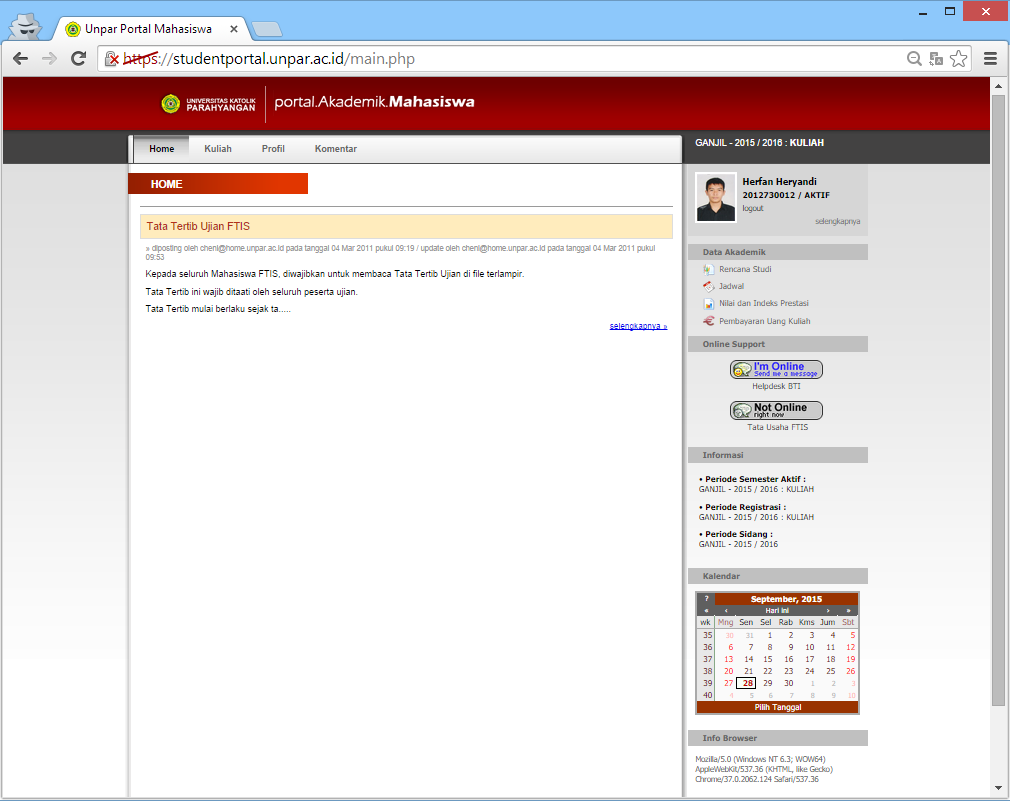
\includegraphics[scale=0.5]{Gambar/pam-home}
	\caption{Halaman Utama Portal Akademik Mahasiswa} 
	\label{fig:3_pam_home}
\end{figure}

Pada halaman utama Portal Akademik Mahasiswa (gambar \ref{fig:3_pam_home}), terdapat beberapa bagian yaitu:
\begin{enumerate}
	\item Menu Atas\\
	Menu ini berfungsi sebagai menu pendukung yang terdiri dari : 
	\begin{itemize}
		\item \textbf{Home}, menampilkan informasi atau pengumuman yang dikeluarkan oleh fakultas masing-masing (Gambar \ref{fig:3_pam_atas_home}). 
		
		\begin{figure}[H]
			\centering
			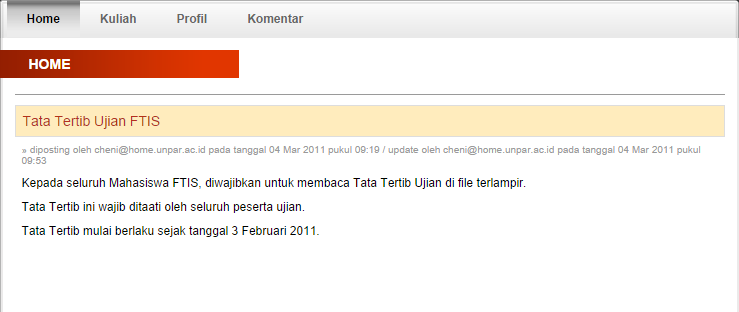
\includegraphics[scale=0.5]{Gambar/pam-atas-home}
			\caption{Menu Atas Home} 
			\label{fig:3_pam_atas_home}
		\end{figure}
		
		\item \textbf{Kuliah}, menampilkan pengumuman per mata kuliah sesuai dengan mata kuliah dan kelas yang diambil oleh masing-masing mahasiswa (Gambar \ref{fig:3_pam_atas_kuliah}).  
		
		\begin{figure}[H]
			\centering
			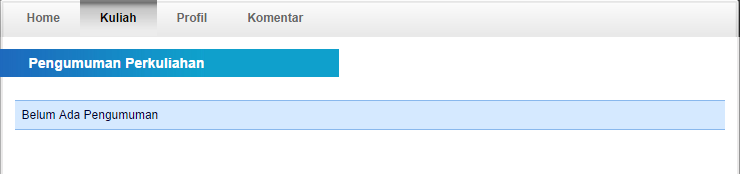
\includegraphics[scale=0.5]{Gambar/pam-atas-kuliah}
			\caption{Menu Atas Kuliah} 
			\label{fig:3_pam_atas_kuliah}
		\end{figure}
		
		\item \textbf{Profil}, berisi tentang data diri masing-masing mahasiswa (Gambar \ref{fig:3_pam_atas_profil}). 
		
		\begin{figure}[H]
			\centering
			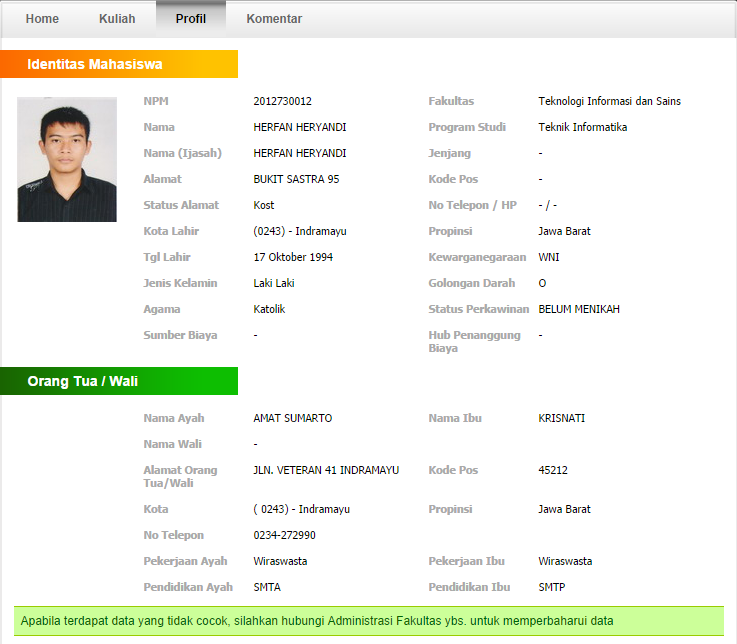
\includegraphics[scale=0.5]{Gambar/pam-atas-profil}
			\caption{Menu Atas Profil} 
			\label{fig:3_pam_atas_profil}
		\end{figure}
		
		\item \textbf{Komentar}, berisi komentar, saran, dan kritik dari mahasiswa (Gambar \ref{fig:3_pam_atas_komentar}).
		
		\begin{figure}[H]
			\centering
			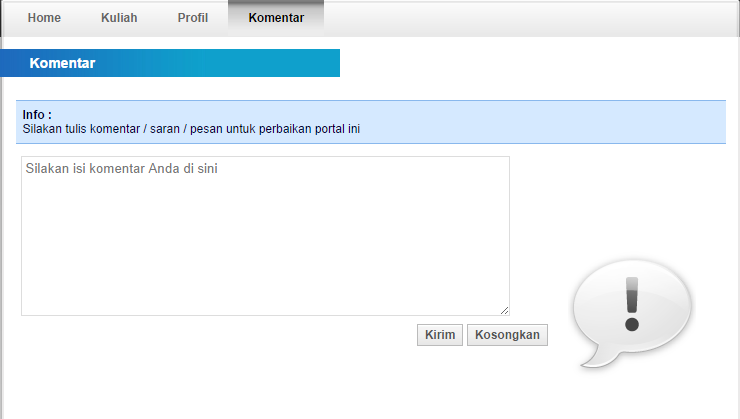
\includegraphics[scale=0.5]{Gambar/pam-atas-komentar}
			\caption{Menu Atas Komentar} 
			\label{fig:3_pam_atas_komentar}
		\end{figure}

	\end{itemize}
	
	\item Identitas Portal \\
	Bagian ini menampilkan identitas pengguna portal. Tampilan identitas ini dapat ditampilkan lengkap dengan melakukan klik pada \textit{link} ``selengkapnya'' atau ditampilkan minimal dengan klik \textit{link} ``tutup''. Identitas yang ditampilkan adalah nama, Nomor Pokok Mahasiswa (NPM), status keaktifan, pas foto, email, dosen wali, program studi, dan fakultas seperti yang terlihat pada gambar \ref{fig:3_pam_identitas}.   
	\begin{figure}[H]
			\centering
			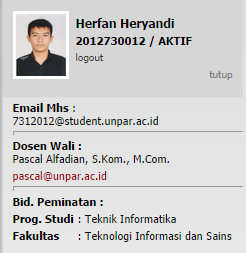
\includegraphics[scale=0.75]{Gambar/pam-identitas}
			\caption{Identitas Portal} 
			\label{fig:3_pam_identitas}
		\end{figure}
		
	\item Menu Utama\\
	Bagian ini memuat fitur utama Portal Akademik Mahasiswa mengenai data akademik (gambar \ref{fig:3_pam_utama}) yang terdiri dari:
		\begin{figure}[H]
			\centering
			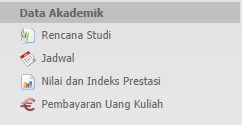
\includegraphics[scale=0.75]{Gambar/pam-utama}
			\caption{Menu Utama} 
			\label{fig:3_pam_utama}
		\end{figure}
	\begin{itemize}
	
		\item \textbf{Rencana Studi}\\
		Menu Rencana Studi terdiri dari submenu: 
		\begin{itemize}
			\item Registrasi (FRS/PRS)\\
			Digunakan sebagai formulir pengisian rencana studi awal (FRS) dan perubahan rencana studi (PRS). 
			\item Kartu Rencana Studi \\
			Menampilkan informasi mata kuliah yang telah diambil melalui submenu Registrasi. Kartu Rencana Studi juga dapat dicetak melalui submenu ini. 
			\item Pindah Kelas MKU \\
			Mahasiswa dapat memilih kelas yang masih tersedia di kolom Jadwal Baru dan menekan tombol ``Simpan'' untuk setiap kelas yang diubah. 
		\end{itemize}
		
		\item \textbf{ Jadwal}\\
		Menu Jadwal terdiri dari submenu: 
		\begin{itemize}
			\item Kuliah, UTS dan UAS \\
			Submenu ini berisi tentang jadwal kuliah, UTS dan UAS yang bisa yang disusun per semester. 
			\item MKU \\
			Submenu ini menampilkan seluruh jadwal Mata Kuliah Umum (MKU) yang memberikan informasi tentang kelas-kelas yang dibuka oleh Pusat Kajian Humaniora (PKH). 
			\item Seluruh Fakultas \\
			Fitur ini memberikan informasi mengenai jadwal-jadwal yang ada di seluruh fakultas.
		\end{itemize}
		
		\item \textbf{Nilai dan Indeks Prestasi}\\
		Menu Nilai dan Indeks Prestasi terdiri dari submenu: 
		\begin{itemize}
			\item Riwayat per Semester \\
			Submenu ini menampilkan informasi nilai per semester. Mahasiswa dapat melihat nilai sesuai dengan semester yang dipilih atau bisa memilih
pilihan ``Seluruh Tahun Akademik'' untuk melihat seluruh nilai berdasarkan semester.
			\item Daftar Perkembangan Studi \\
			Seluruh riwayat mata kuliah dan nilai yang pernah ditempuh ditampilkan di submenu ini. Pada bagian bawah halaman, terdapat statistik nilai dan indeks prestasi. 
			\item Riwayat Indeks Prestasi \\
			Menampilkan daftar riwayat indeks prestasi semester dan kumulatif setiap semester. Tampilan ini juga dilengkapi dengan grafik perkembangan. 
			\item TOEFL \\
			Menampilkan daftar riwayat skor \textit{Test of English as Foreign Language} (TOEFL) yang pernah ditempuh. Mahasiswa diwajibkan untuk menempuh TOEFL dengan skor minimal 500.
		\end{itemize}
		
		\item \textbf{Pembayaran Uang Kuliah}\\
		Menu ini berfungsi untuk melihat data tagihan pembayaran uang kuliah serta cara-cara pembayarannya.
		\end{itemize}
		
	\item \textbf{Informasi}\\
		Bagian ini menampilkan informasi tentang periode-periode yang sedang aktif.
		
	\item \textbf{Kalender}\\
		Bagian ini menampilkan kalender masehi.
		
	\item \textbf{Info Browser}\\
		Bagian ini menampilkan informasi tentang internet \textit{browser} yang digunakan pada saat membuka Portal Akademik Mahasiswa. 
\end{enumerate}

\section{Analisis Kebutuhan IT Student Portal}
Dalam menganalisis kebutuhan IT Student Portal, penulis melakukan wawancara dengan 18 mahasiswa Program Studi Teknik Informatika UNPAR. Kriteria dari 18 mahasiswa tersebut yaitu lipsum. Setelah melakukan wawancara, penulis memperoleh fitur-fitur yang dibutuhkan antara lain:
\begin{enumerate}
	\item Prasyarat mata kuliah
	\item Status perkuliahan
	\item DPS dapat berubah sesuai riwayat nilai
	\item Susunan jadwal terurut
	\item Detail Kuliah
	\item Tampilan \textit{desktop} pada sistem operasi selain Windows 
	\item Daftar email dosen
	\item Upload CV
\end{enumerate}
Fitur-fitur yang akan dipilih harus memenuhi kriteria:
\begin{itemize}
	\item Dibuat untuk mempermudah penggunaan Student Portal
	\item Didukung Student Portal
\end{itemize}
Berdasarkan kriteria di atas dan batas waktu pembangunan aplikasi, maka akan dipilih fitur-fitur sebagai berikut:
\begin{enumerate}
	\item Prasyarat mata kuliah
	\item Susunan jadwal yang terurut 
	\item Tampilan \textit{desktop} pada sistem operasi selain Windows
\end{enumerate}


\section{Analisis Komunikasi Portal Akademik Mahasiswa untuk Fitur IT Student Portal}
Student Portal UNPAR diakses dengan melakukan request pada URL \url{https://studentportal.unpar.ac.id/}. Saat mengklik tombol \textit{login}, halaman akan melakukan \textit{request} ke URL \url{https://studentportal.unpar.ac.id/home/index.login.submit.php} dengan mengirim Form Data \texttt{Submit=Login}. Halaman yang diperoleh dari pengiriman tersebut adalah halaman CAS UNPAR. Di halaman CAS UNPAR, \textit{login} akan dilakukan dengan mengirimkan data \texttt{username} yang berisi email \textit{student} UNPAR, \texttt{password} berisi kata sandi dari email \textit{student} UNPAR, \texttt{lt} diperoleh dari nilai elemen \texttt{input} dengan nama ``lt'', execution diperoleh dari nilai elemen \texttt{input} dengan nama ``execution'', dan \texttt{\_eventId} berisi ``submit"'. Setelah data tersebut dikirim ke URL \url{https://cas.unpar.ac.id/login}, akan diperoleh respon halaman depan Student Portal UNPAR dan \textit{cookies}.
